\documentclass{article}
\usepackage{graphicx}
\usepackage[hidelinks]{hyperref}
\usepackage{enumitem}
\usepackage{array}
\usepackage{amsmath}
\usepackage{float}
\usepackage[
    top=2.5cm,
    bottom=2.5cm,
    left=2.5cm,
    right=2.5cm,
    headheight=14pt  % prevents warnings
]{geometry}

\usepackage{setspace}
\setstretch{1.1}  % 10% more than single spacing

\title{\textbf{CS310 Project Specification:\\
GiTrip\\
\vspace{-1.5mm}
$\sim$ \textit{Git} for Collaborative Trip Planning $\sim$}}
\author{Tatsunori Ono}
\date{October 2025}

\begin{document}
\maketitle

\section{Problem Statement}

Trip planning is time-consuming because we must consider many factors, such as travel time, the mode of transportation, the opening and closing times of each stop, and other logistical details. The process becomes even more complicated when it comes to a group trip, as it involves messaging, sharing documents and map screenshots. When itineraries change, participants make parallel edits. It is highly likely to lose track of who changed what, when, and why, and it is difficult to ``try ideas'' because edits can overwrite each other. Existing tools either optimise a single itinerary (e.g., \textit{Google Maps}) or support generic collaboration (e.g., \textit{Notion} and \textit{Google Docs}), but they often treat change management as an afterthought. This leads to duplicated plans, time clashes, missed opening hours, and a lack of backup options.

\textit{GiTrip} addresses this problem by applying \textit{Git}\cite{git}-style version control to trip planning. Users initialise a \emph{trip repository}, branch to explore alternative trip plans, and merge them with structured conflict resolution. A built-in automatic scheduler reorders stops to reduce travel time and enforces constraints such as daily active hours, per-stop stay duration, opening-hours windows, and user preferences (compact vs. sparse, morning/midday/night focus, transport mode, and so on). \textit{GiTrip} fully visualises trip plans through two approaches. One is via an interactive timeline, which users can adjust times by dragging handles, and it automatically
calculates the travel time between successive stops to keep the schedule optimised. Second is via graphs (typically a DAG --- Directed Acyclic Graph) on a per-day map.

As a specific use case, a group of friends can initialise a shared repository for their London trip. Then, they can branch it so that each person can edit the trip plan as they like (e.g., museum-route and food-route). Finally, they can merge the trip plans into one by resolving conflicts, such as overlapping time, to finalise their London trip. Alternatively, users can rollback to any previous version if plans change. They can also fork and customise public trip repositories created by others.

This project is suitably challenging for a 3rd-year Computer Science project since it requires integration of Version Control System (VCS) semantics on a constraint-based scheduling with external routing services, and visualising it through an interactive UI of timeline \& map editing.

\section{Objectives}

The aim of \textit{GiTrip} is to turn trip planning into a clear, flexible, and easy process. The following are MoSCoW (must-have, should-have, could-have, and will-not-have right now as there is not enough time) prioritisation of each feature to accomplish the objective efficiently:

\subsection*{Must-haves (M)}
\begin{enumerate}[label=\textbf{M\arabic*}]
  \item \textbf{Trip repositories with history:} Record of commits, branches, and all snapshot history (in JSON files). Visualisation of the trip repository history via a workflow diagram (a graph representing branches and merging). This user-friendly visualisation allows all users to intuitively use the application even if they are not familiar with \textit{Git}.
  \item \textbf{Optimised automatic scheduler:} User input places, stay durations, strict-ordering of places, desired windows, daily active hours, break minutes, target day range, and user preferences. Then, output a non-overlapping plan across one or more days, considering all constraints.
  \item \textbf{Routing data integration:} Data for travel time will be retrieved using \textit{Openrouteservice} and \textit{Google Directions}, then fed into the automatic scheduler.
  \item \textbf{Interactive visualisation:} Trip timeline (with dotted segments to show travel gaps) and DAG map (with ordered markers with numbers). Edits commit back to the repository.
  \item \textbf{Merge and conflicts:} Merge operation for plan JSON (stop/field granularity) with a conflict resolver screen.
\end{enumerate}

\subsection*{Should-haves (S)}
\begin{enumerate}[label=\textbf{S\arabic*}]
  \item \textbf{User input validation:} Opening-hours validation with automatic nudge to nearest feasible slot.
  \item \textbf{User preferences setting:} Compact vs.\ sparse scheduling; morning/midday/night focus; recompute travel by mode (driving/walking/cycling/transit).
  \item \textbf{Branch productivity:} Create branch from Web UI, compare branches, and fork plan from a public repository.
\end{enumerate}

\subsection*{Could-haves (C)}
\begin{enumerate}[label=\textbf{C\arabic*}]
  \item \textbf{Command-line interface (CLI) along with the Web UI:} \textit{Git}-style operations can be performed on the Web UI through clear navigation of buttons. Additionally, the \texttt{gitrip} terminal commands, such as \texttt{gitrip init/add/commit/push/branch/merge} on \textit{GiTrip} CLI, provide the same operations as the Web UI.
  \item \textbf{Public trip repository:} Public repository gallery with attribution and one-click fork.
  \item \textbf{Real-time tracking:} Live GPS guidance during travel to detect running late, suggest reflow, and show original vs. updated times.
  \item \textbf{Busy-time consideration:} Take into account the crowd level in the automatic scheduler to avoid peak times.
  \item \textbf{Progressive Web App (PWA):} A Service Worker caches the app's core files so users can view trips offline. When offline, the app allows read-only access to the last-opened repository. Changes made offline are queued and automatically synchronised when the connection returns. Users can install the app like a native application.
\end{enumerate}

\subsection*{Will-not-haves (W)}
These are out of scope for the Minimum Viable Product (MVP) but are acknowledged and designed for future improvements.
\begin{enumerate}[label=\textbf{W\arabic*}]
  \item \textbf{Real-time collaborative editing:} While multiple users can work on branches and merge later, simultaneous live editing with operational transforms is out of scope.
  
  \item \textbf{Booking/reservation integration:} \textit{GiTrip} plans trips but does not interface with hotel, restaurant, or ticket booking systems.

  \item \textbf{Budget tracking and expense splitting:} Financial features (cost estimates, shared expenses, currency conversion) are deferred to specialised tools for now.
  
  \item \textbf{Social features (chat, reviews, ratings):} Communication happens outside the app. \textit{GiTrip} focuses on version-controlled planning, not social networking.
  
  \item \textbf{Mobile native apps (iOS/Android):} The PWA approach provides cross-platform access. Native Swift/Kotlin apps require resources beyond the current scope.
  
  \item \textbf{AI-powered itinerary generation from natural language:} For example, ``plan a romantic weekend in Paris". The auto-scheduler requires structured input, and LLM integration is future work.

  \item \textbf{Learning \& Smart Assistance:} While this project prioritises deterministic scheduling, there is a potential for learning user preferences (e.g., morning person, tolerance for long transfers) to bias the auto-scheduler or recommend places/routes from past trips.\\
\end{enumerate}

\subsection{Success Criteria}
\begin{enumerate}
  \item Create two alternative plans, merge, and resolve at least one timing conflict in $<5$ minutes on average by 80\% of 10--30 test participants.
  \item Automatic scheduler produces a non-overlapping sequence of activities for $\ge 6$ stops across 1--2 days with non-zero, realistic travel gaps.
  \item No critical issues with accessibility and follows \textit{Web Content Accessibility Guidelines (WCAG) 2.2}\cite{wcag22}.
\end{enumerate}

\section{Technical and Concept}

\subsection{System Overview}
\begin{itemize}
  \item \textbf{Backend (Node.js \& Express):} The server handles trip data, version control logic, and API requests. Each commit stores a snapshot with \textit{plan.json} describing the itinerary. Using JSON for plans makes merging straightforward and avoids complex database migrations\cite{json-merge-patch}.
  
  \item \textbf{Frontend (EJS templates):} Server-rendered HTML pages provide the web interface. The timeline is drawn as an SVG graphic with drag handles for adjusting times. Maps use \textit{Leaflet} (an open-source mapping library) to show numbered location pins connected by routes line, forming a DAG. When conflicts occur, users see side-by-side comparisons and choose which version to keep for each field.
  
  \item \textbf{Database (SQLite):} A lightweight file-based database stores the core data of trip repositories, branches, commits (snapshots of changes), and snapshots (the actual trip data at each commit).
  
  \item \textbf{Web Server (Nginx):} Handles incoming HTTP requests, serves static files, and forwards dynamic requests to the Node.js backend.
\end{itemize}

\subsection{Place Search and Opening-hours}
Place search uses \textit{OpenStreetMap} and \textit{Nominatim} by a server-side proxy that sets a compliant user-agent, handles requests, and returns coordinates with \texttt{opening\_hours} if available. Opening-hours strings are parsed and validated. When the requested stay does not fit the daily window, the scheduler nudges to the next feasible interval or rolls forward to the next day.

\subsection{Routing}
If coordinates are available, \textit{GiTrip} calls:
\begin{itemize}
  \item \textbf{\textit{Openrouteservice} (ORS)} for matrix endpoint\cite{ors-matrix} or per-leg (one segment of travel between two consecutive stops) routing in driving, walking, and cycling modes.
  \item \textbf{\textit{Google Directions}} for transit (sequential legs).
\end{itemize}
When APIs are unavailable, haversine distance estimates minutes per leg with mode-specific min/km constants. All calls occur server-side and keys are never exposed to the browser.

\subsection{Optimisation strategy and limits}
Ordering uses nearest-neighbour (NN) over a duration matrix when available from ORS; otherwise haversine distance. This heuristic is $O(n^2)$ and performs well for $n\le 50$ stops\cite{hougardy-nn}. Exact TSP (Travelling Salesman Problem)\cite{applegate-tsp} or meta-heuristics\cite{johnson-mcgeoch} are intentionally avoided to fit module scope and API quotas.

For large itineraries (more than 50 stops or spanning more than 10 days), \textit{GiTrip} divides the trip into day-sized chunks, optimises each day independently, then calculates travel times between the last stop of each day and the first stop of the next.

When users manually adjust stop times by the timeline editor, those stops are locked to their chosen times. Subsequent auto-rescheduling preserves locked times and only adjusts neighbouring stops to maintain feasibility (e.g., ensuring no overlaps and respecting travel durations).

\subsection{Scheduling Model}
Given ordered stops $S_1,\dots,S_n$, per-leg travel $T_i$ (minutes from $S_{i-1}$ to $S_i$), stay durations $D_i$, active window $[A,B]$, break $b$, and focus offset $f$:
\[
a_1 = A+f,\quad d_1=a_1+D_1,\quad
a_i = d_{i-1}+b+T_i,\quad d_i=a_i+D_i \ (i>1).
\]
If $(a_i,d_i)$ violates desired window or opening-hours, the scheduler shifts to the nearest valid interval inside $[A,B]$; otherwise, it spills to the next day's $A+f$\cite{timetable-scheduling}. The user preference, compact vs.\ sparse, controls additional free time after each stop. The output is a list of days with ordered stops and their arrive/depart times.

\subsection{Versioning and Merge}

Each commit saves who made the change, a description message, links to parent commits, and a complete snapshot of the trip at that point in time. Trip plans (\texttt{plan.json}) are merged by matching stops using their unique IDs. If two people changed different aspects of the same stop (e.g., one changed arrival time, another changed duration), \textit{GiTrip} shows both versions and asks the user to choose. The system then creates a new snapshot combining the chosen changes.

\subsection{Conflict Resolution}

When merging two versions of a trip, \textit{GiTrip} compares them against their common starting point (the last version both people had before making changes). The system handles several types of conflicts:
\begin{itemize}
  \item \textbf{Field conflicts:} When both users edit the same field, \textit{GiTrip} shows both versions with a preview timeline for field-by-field resolution.
  
  \item \textbf{Timing conflicts:} After merging, \textit{GiTrip} flags timing issues (overlapping stops, insufficient travel time) and offers automatic rescheduling or manual adjustment.
  
  \item \textbf{Multi-way merges:} Combined by merging pairs sequentially, with each step tracked.
  
  \item \textbf{Simultaneous edits:} If two people push changes simultaneously, the second person receives a notification and must walk through an interactive merge process before their changes can be saved.
\end{itemize}

If the merged trip is logically impossible (e.g., overlapping times, impossible travel), \textit{GiTrip} allows the commit but marks it with an ``infeasible'' warning. Again, the next screen offers to automatically fix the schedule or let you adjust it manually.

\subsection{Collaboration}
Each repository has an owner and collaborators with roles: viewer (read), contributor (commit/push/branch), maintainer (merge/protect branches). Protected branches (e.g., \texttt{main}) require maintainer role to merge.

\section{Methodology}

A waterfall approach with weekly milestones and demos to the supervisor will be used. Biweekly (once in 2 weeks) in-person supervision meetings with Professor Mike Joy are scheduled throughout the project duration (Week 2, Week 4,  \dots, Week 26 - excluding vacations). When needed, there will be extra meetings. For example, this time we had one extra meeting in Week 1 for checking the first draft of this project specification.

\subsection{Testing}
We will use the following testing for specific parts of the project:
\begin{itemize}
    \item \textbf{Unit:} Testing for opening-hours parser, time arithmetic, merge functions, and CLI command parsing.
    \item \textbf{Integration:} Testing for end-to-end auto-plan with mocked routing, and push/merge conflict workflows.
    \item \textbf{User Acceptance Testing (UAT):} Testing for User Experience (UX) on each feature by referring to Nielsen's usability heuristics\cite{nielsen-usability} as a criterion. This will be conducted through a survey with participants on Evaluation Day, measuring task completion time, error rates, and user satisfaction scores.
\end{itemize}

\section{Timetable}

\textit{Figure 1} shows the Gantt chart of this project, and \textit{Figure 2} denotes the colour-coded keys for it. Some tasks are scheduled to run in parallel based on their complexity. The Christmas vacation serves as a buffer period, allowing time for coursework and personal rest. The Easter vacation falls close to the final report deadline, hence writing up and rehearsal are scheduled during this period to maintain progress.

\begin{figure}[H]
\centering
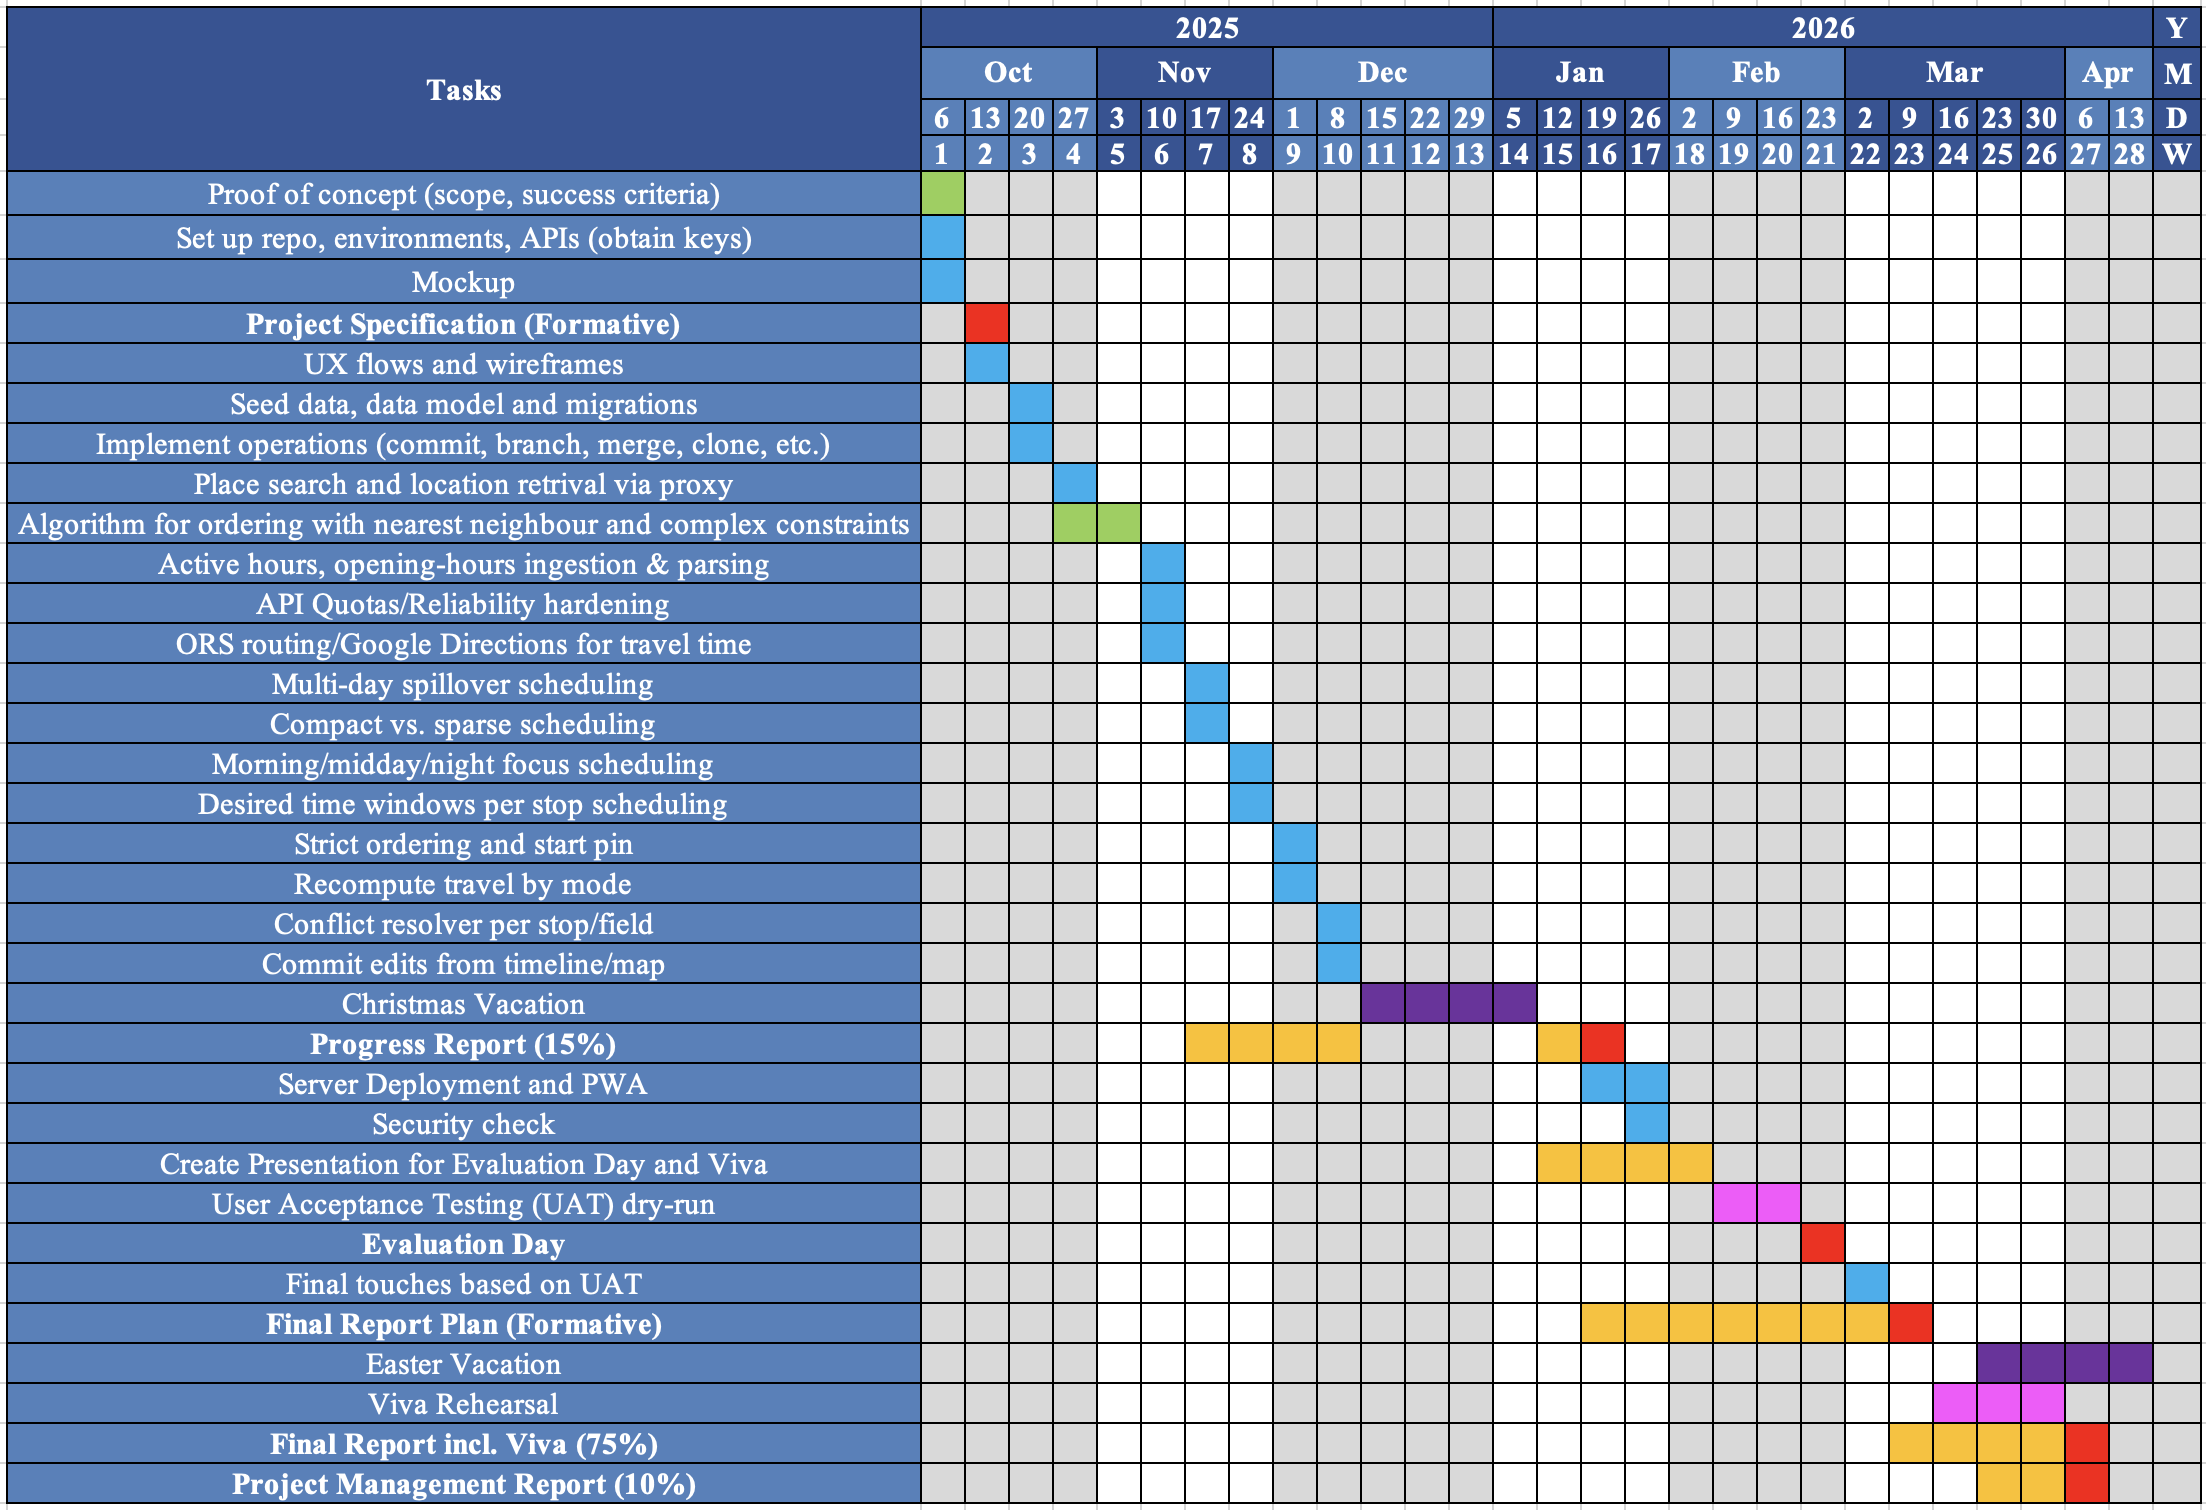
\includegraphics[width=\textwidth]{gantt.png}
\caption{Project Gantt Chart}
\end{figure}

\begin{figure}[H]
\centering
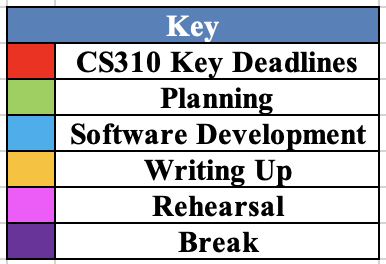
\includegraphics[width=0.3\textwidth]{key.png}
\caption{Gantt Chart Key}
\end{figure}

\section{Resources}
\begin{itemize}
    \item \textit{OpenStreetMap}/\textit{Nominatim} data for place search
    \item \textit{Openrouteservice} (free) and \textit{Google Directions} for routing
    \item \textit{GitHub} for version control
    \item \textit{Overleaf} for documentation
    \item \textit{Vercel} (free) for deployment
\end{itemize}

\subsection{Risks and Mitigations}

\begin{itemize}
  \item \textbf{API quotas and outages:} Server proxy with throttle and caching; haversine distance calculation as a fallback ensures the continuity of scheduler.
  \item \textbf{API key leakage:} Store keys in server env vars only; never ship to client. Rotate keys on suspected exposure; restrict by referrer/IP where supported.
  \item \textbf{Supervisor illness/extended absence or change of supervisor:} Maintain concise weekly status notes and a living roadmap so handover is trivial. Switch to remote supervision if needed. If unavailable for $>$2 weeks, ask the module organiser to assign an interim supervisor; continue against approved milestones. 
  \item \textbf{Student illness:} Build buffers into schedule and adjust MoSCoW prioritises. If it is a serious health issue, file mitigating circumstances and agree a recovery plan at next check-in.
  \item \textbf{Hardware for local development lost/theft:} Manage project repository privately on \textit{GitHub} with 2FA; push at least daily.
  \item \textbf{Data loss or corruption:} Commit frequently and keep a protected \texttt{main} branch.
\end{itemize}

\section{Legal, Social, Ethical and Professional Issues \& Considerations}

\textit{GiTrip} minimises personal data collection and mainly stores trip content, such as places and dates/times. Users can export or delete their data upon request, following GDPR principles. When using external services, the application follows the provider's terms and attribution requirements for \textit{OpenStreetMap}, \textit{Openrouteservice}, and \textit{Google Directions}. Publicly shared plans must adhere to a brief Terms of Service, which includes rules against abusive content or unlawful use, along with a simple reporting system for inappropriate names or descriptions. For UAT, people at Evaluation Day (students and staff from the University of Warwick Department of Computer Science), my friends, and my family will be participating. Therefore, ethical consent is not required. Accessibility meets \textit{WCAG 2.2} guidance, including keyboard operation, screen-reader labels, and adequate colour contrast.

\begin{thebibliography}{9}

\bibitem{git}
L.~Torvalds and J.~C.~Hamano, ``Git: distributed version control system,'' 2005--2025.
[Online]. Available: \url{https://git-scm.com/}. [Accessed: 1 Jun. 2025].

\bibitem{wcag22}
W3C, \emph{Web Content Accessibility Guidelines (WCAG) 2.2}, Oct.\ 2023.
[Online]. Available: \url{https://www.w3.org/TR/WCAG22/}. [Accessed: 7 Oct. 2025].

\bibitem{json-merge-patch}
J.~K.~Nottingham and P.~Bryan, ``RFC 7396: JSON Merge Patch,'' IETF, 2014.
doi: \href{https://doi.org/10.17487/RFC7396}{10.17487/RFC7396}.

\bibitem{ors-matrix}
Openrouteservice, ``Matrix Endpoint — API Reference,'' Sept.\ 2025.
[Online]. Available: \url{https://giscience.github.io/openrouteservice/api-reference/endpoints/matrix/}.
[Accessed: 8 Oct. 2025].

\bibitem{hougardy-nn}
S.~Hougardy, ``On the nearest neighbor rule for the metric traveling salesman problem,''
\emph{Discrete Applied Mathematics}, vol.~187, pp.~62--72, 2015.
doi: \href{https://doi.org/10.1016/j.dam.2015.03.002}{10.1016/j.dam.2015.03.002}.
[Online]. Available: \url{https://www.sciencedirect.com/science/article/pii/S0166218X14001486}.
[Accessed: 9 Oct. 2025].

\bibitem{applegate-tsp}
D.~L.~Applegate, R.~E.~Bixby, V.~Chv\'atal, and W.~J.~Cook,
\emph{The Traveling Salesman Problem: A Computational Study}.
Princeton, NJ, USA: Princeton University Press, 2007.
ISBN: 978-0-691-12993-8.

\bibitem{johnson-mcgeoch}
D.~S.~Johnson and L.~A.~McGeoch, ``The Traveling Salesman Problem: A Case Study in Local Optimization,''
in \emph{Local Search in Combinatorial Optimization}. Chichester, UK: Wiley, 1997.
[Online]. Available: \url{https://www.cs.ubc.ca/~hutter/previous-earg/EmpAlgReadingGroup/TSP-JohMcg97.pdf}.
[Accessed: 9 Oct. 2025].

\bibitem{timetable-scheduling}
E.~K.~Burke and H.~Rudov\'a, Eds., \emph{Practice and Theory of Automated Timetabling VI (PATAT 2006)}.
Berlin, Germany: Springer, 2007. ISBN: 978-3-540-77345-0.

\bibitem{nielsen-usability}
J.~Nielsen, \emph{Usability Engineering}. San Francisco, CA, USA: Morgan Kaufmann, 1994.
ISBN: 978-0-12-518406-9.

\end{thebibliography}


\end{document}
